\phantomsection
\section*{Manual de Usuario}
\addcontentsline{toc}{section}{Manual de Usuario}

Este manual proporciona una guía básica para el uso de la aplicación, explicando las funcionalidades disponibles y cómo acceder a ellas.

\subsection*{1. Inicio de la aplicaci\'on}
Al ejecutar la aplicación, se muestra una pantalla de inicio de sesión con opciones para iniciar sesión o registrarse.

\begin{figure}[H]
    \centering
    \includegraphics[width=0.6\textwidth]{images/manualDeUsuario/InicioAplicación.png}
    \caption*{Pantalla de inicio de sesión}
\end{figure}

\subsection*{2. Registro de un nuevo usuario}
Para crear una cuenta, el usuario debe seleccionar la opción \texttt{Register} y completar el formulario.

\begin{itemize}
    \item Introducir el número de teléfono, nombre de usuario y contraseña.
    \item Para modificar la imagen de perfil, introducir la url de la imagen deseada, y pulsar el botón de la derecha.
    \item Pulsar el botón \texttt{register}.
\end{itemize}

\begin{figure}[H]
    \centering
    \begin{minipage}[b]{0.48\textwidth}
        \centering
        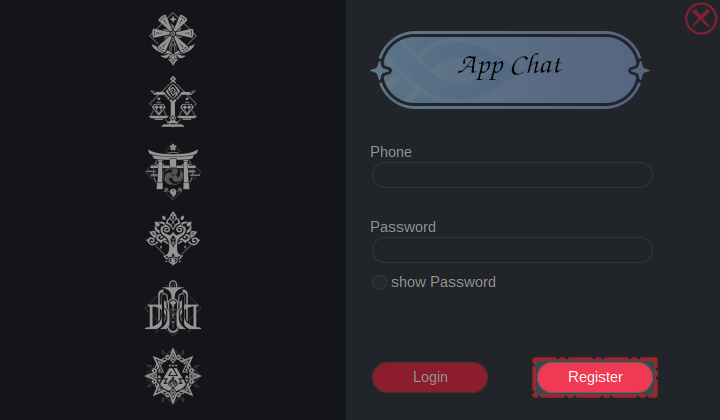
\includegraphics[width=\textwidth]{images/manualDeUsuario/registro1.png}
        \caption*{Formulario de registro - Parte 1}
    \end{minipage}
    \hfill
    \begin{minipage}[b]{0.48\textwidth}
        \centering
        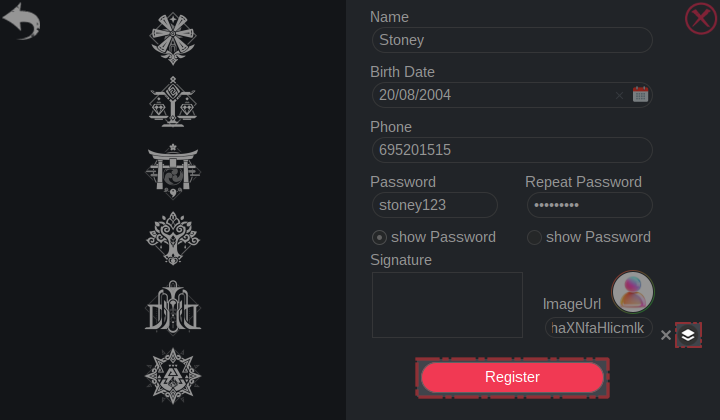
\includegraphics[width=\textwidth]{images/manualDeUsuario/registro2.png}
        \caption*{Formulario de registro - Parte 2}
    \end{minipage}
\end{figure}

\subsection*{3. Inicio de sesión}
Para iniciar sesión, el usuario debe introducir sus credenciales en la pantalla de inicio de sesión y pulsar el botón \texttt{Login}.

\begin{figure}[H]
    \centering
    \begin{minipage}[b]{0.48\textwidth}
        \centering
        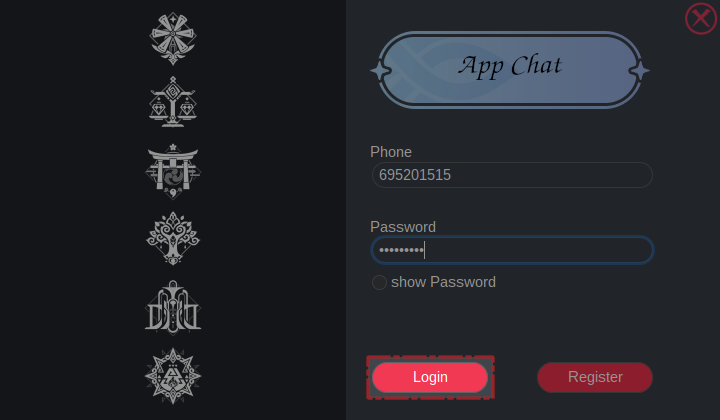
\includegraphics[width=0.96\textwidth]{images/manualDeUsuario/InicioSesion1.png}
        \caption*{Pantalla de inicio de sesión}
    \end{minipage}
    \hfill
    \begin{minipage}[b]{0.48\textwidth}
        \centering
        
\includegraphics[width=\textwidth]{images/manualDeUsuario/InicioSesion2.png}
        \caption*{Pantalla principal}
    \end{minipage}
\end{figure}

Tras iniciar sesión, el usuario accede a la pantalla principal de la aplicación, desde donde puede ver sus contactos y grupos, así como realizar otras operaciones.

\subsection*{4. Añadir un nuevo contacto}
Para añadir un nuevo contacto, el usuario debe pulsar el botón para acceder a la lista de contactos y luego seleccionar la opción \texttt{Add Contact}. 

\begin{figure}[H]
    \centering
    \begin{minipage}[b]{0.48\textwidth}
        \centering
        \includegraphics[width=\textwidth]{images/manualDeUsuario/AñadirContacto1.png}
        \caption*{Botón de contactos}
    \end{minipage}
    \hfill
    \begin{minipage}[b]{0.48\textwidth}
        \centering
        \includegraphics[width=\textwidth]{images/manualDeUsuario/AñadirContacto2.png}
        \caption*{Lista de contactos}
    \end{minipage}
\end{figure}

A continuación, el usuario debe introducir el número de teléfono del contacto, el nombre que desea asignarle y pulsar el botón \texttt{Añadir}.

\begin{figure}[H]
    \centering
    \includegraphics[width=0.58\textwidth]{images/manualDeUsuario/AñadirContacto3.png}
    \caption*{Formulario para añadir contacto}
\end{figure}

\subsection*{5. Crear un nuevo grupo}
Para crear un nuevo grupo, el usuario debe pulsar el botón para acceder a la lista de grupos y luego seleccionar la opción \texttt{Create Group}.

\begin{figure}[H]
    \centering
    \begin{minipage}[b]{0.48\textwidth}
        \centering
        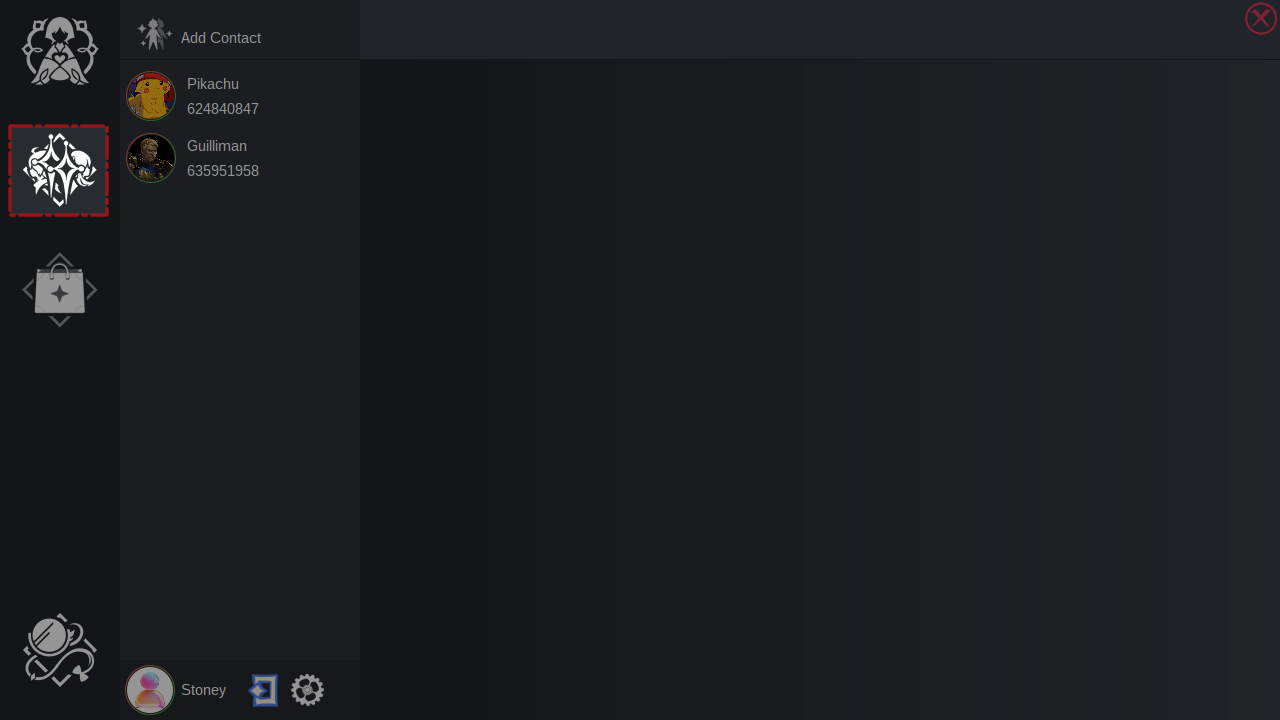
\includegraphics[width=\textwidth]{images/manualDeUsuario/HacerGrupo1.png}
        \caption*{Botón de grupos}
    \end{minipage}
    \hfill
    \begin{minipage}[b]{0.48\textwidth}
        \centering
        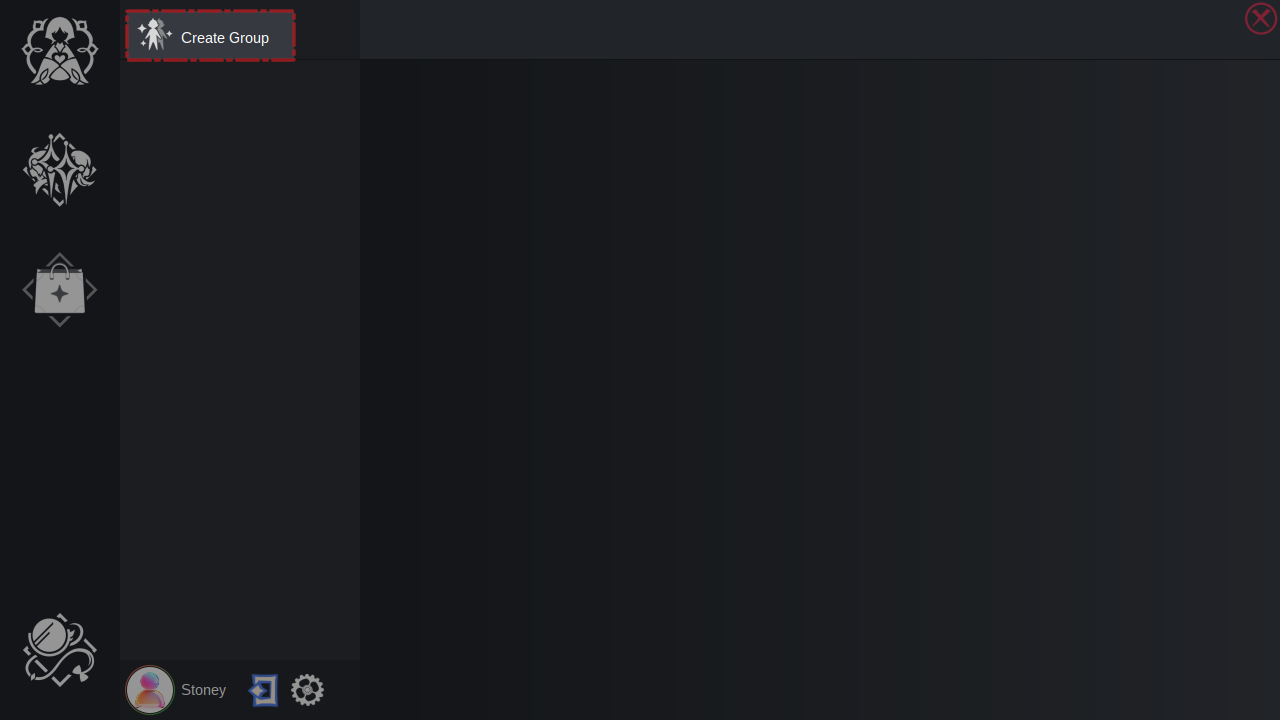
\includegraphics[width=\textwidth]{images/manualDeUsuario/HacerGrupo2.png}
        \caption*{Lista de grupos}
    \end{minipage}
\end{figure}

A continuación, el usuario debe introducir el nombre del grupo y seleccionar los contactos que desea añadir al grupo. Finalmente, debe pulsar el botón \texttt{Accept}.

\begin{figure}[H]
    \centering
    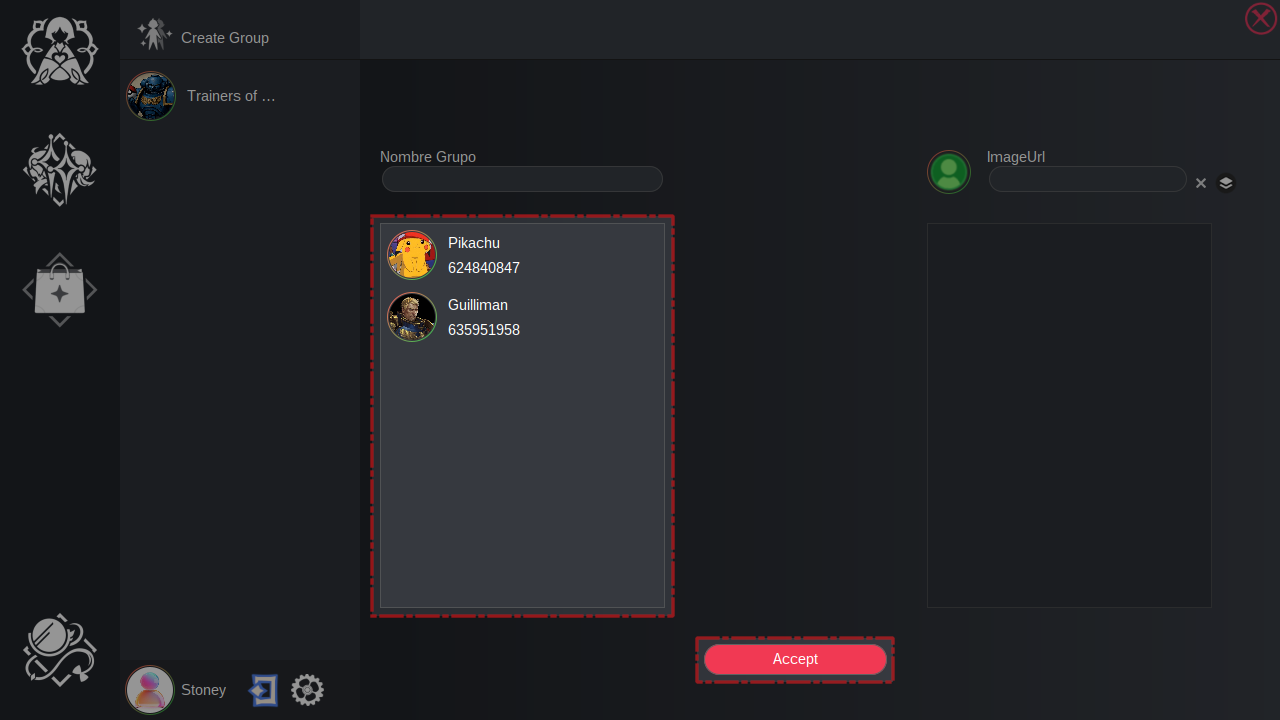
\includegraphics[width=0.58\textwidth]{images/manualDeUsuario/HacerGrupo3.png}
    \caption*{Formulario para crear grupo}
\end{figure}

\subsection*{6. Enviar un mensaje}
Para acceder a la pantalla de chat, el usuario debe seleccionar un contacto o grupo de la lista.
Una vez en la pantalla de chat, el usuario puede enviar mensajes de texto o emojis.

\begin{figure}[H]
    \centering
    \begin{minipage}[b]{0.48\textwidth}
        \centering
        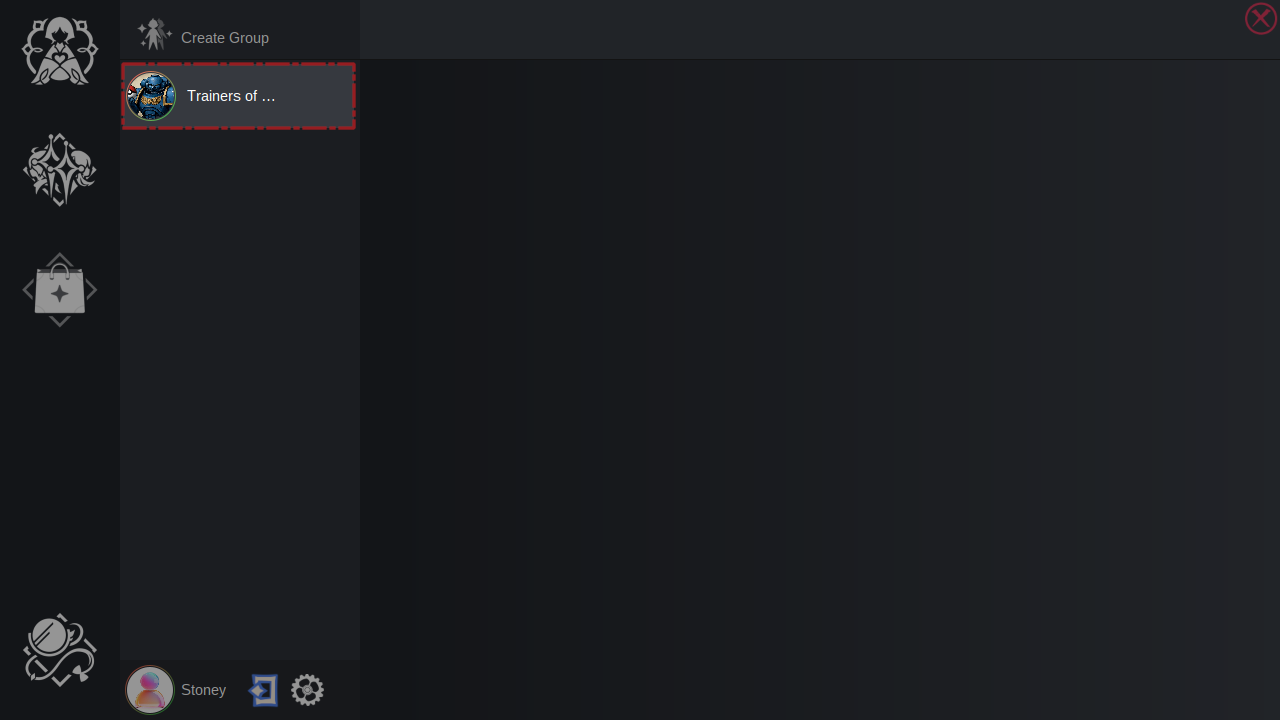
\includegraphics[width=\textwidth]{images/manualDeUsuario/EnviarMensaje1.png}
        \caption*{Lista de grupos}
    \end{minipage}
    \hfill
    \begin{minipage}[b]{0.48\textwidth}
        \centering
        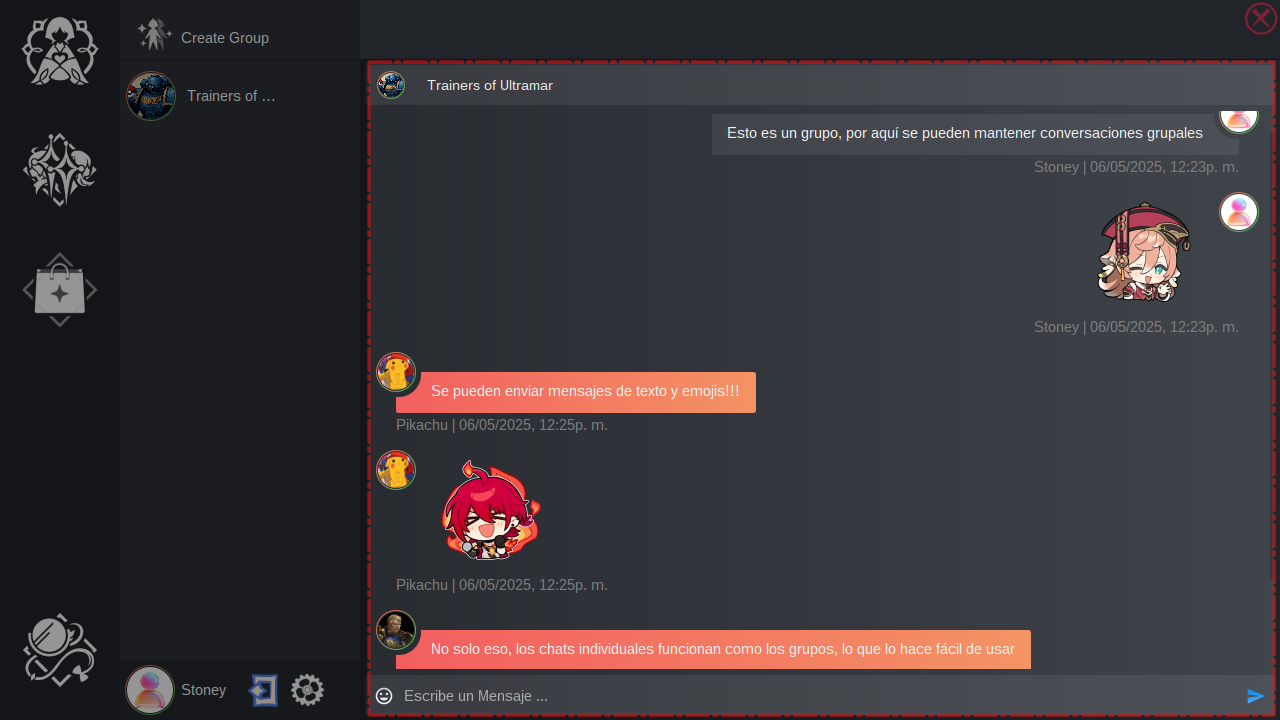
\includegraphics[width=\textwidth]{images/manualDeUsuario/EnviarMensaje2.png}
        \caption*{Pantalla de chat}
    \end{minipage}
\end{figure}

\subsection*{7. Gestionar contactos y grupos}
El usuario puede gestionar sus contactos y grupos desde el menu de ajustes.
Para acceder a los ajustes, el usuario debe pulsar el botón con forma de engranaje en la parte inferior de la pantalla principal.

\begin{figure}[H]
    \centering
    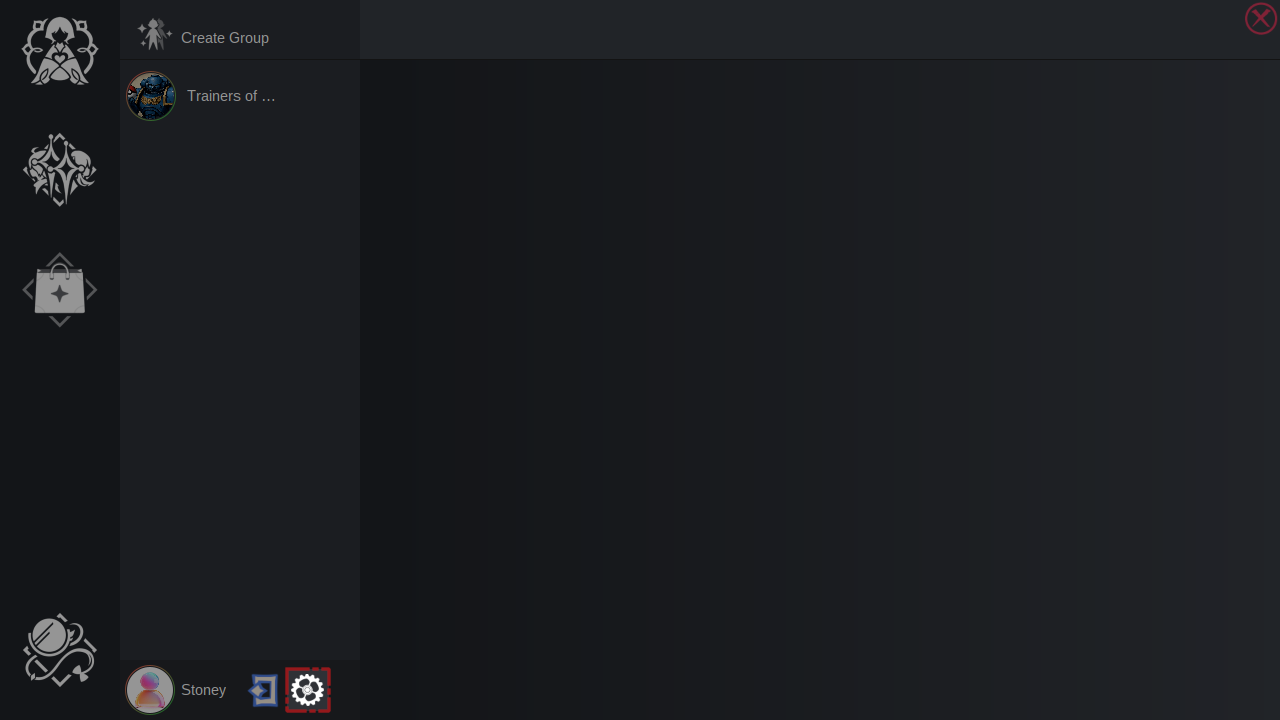
\includegraphics[width=0.58\textwidth]{images/manualDeUsuario/EditarContactos&Grupos1.png}
    \caption*{Botón de ajustes}
\end{figure}

Una vez ahí puede seleccionar un contacto para editar su nombre de contacto o eliminarlo de la lista de contactos.

\begin{figure}[H]
    \centering
    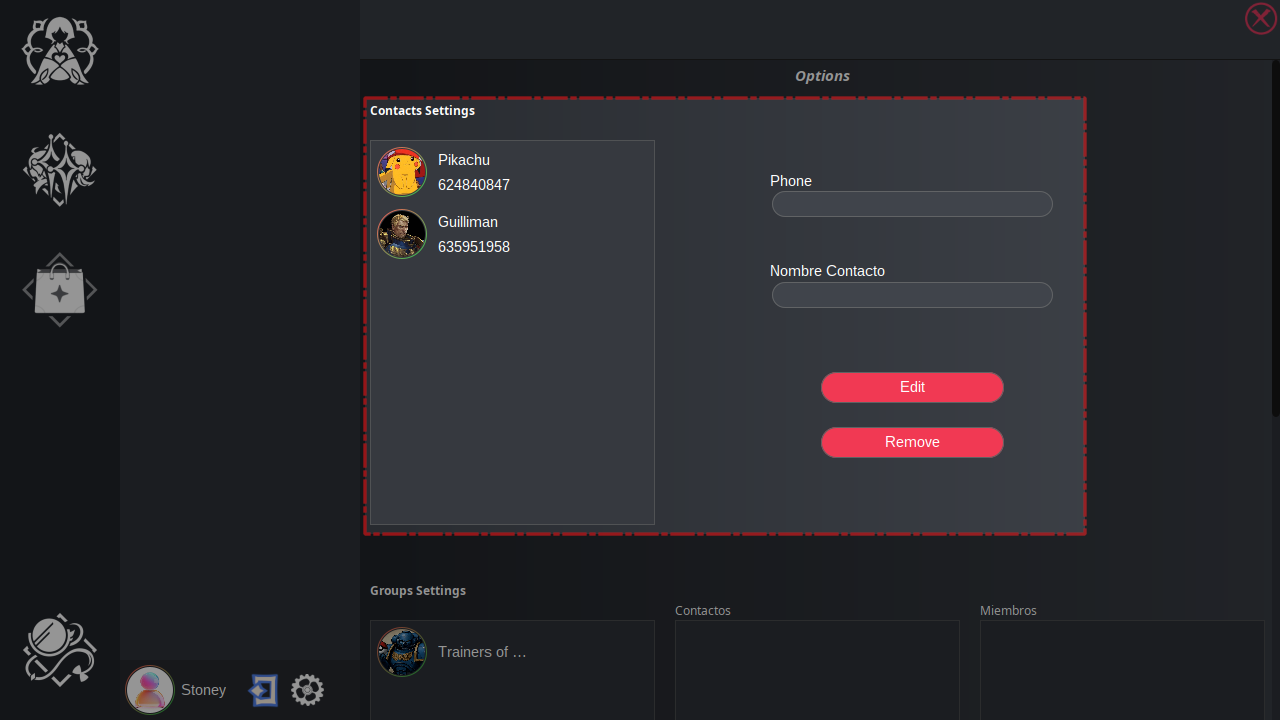
\includegraphics[width=0.58\textwidth]{images/manualDeUsuario/EditarContactos&Grupos2.png}
    \caption*{Ajustes de contactos}
\end{figure}

En el caso de los grupos, solo el administrador del grupo puede eliminarlo o modificar su información, pero no puede abandonar el grupo. 
Los miembros solo pueden abandonar el grupo.

\begin{figure}[H]
    \centering
    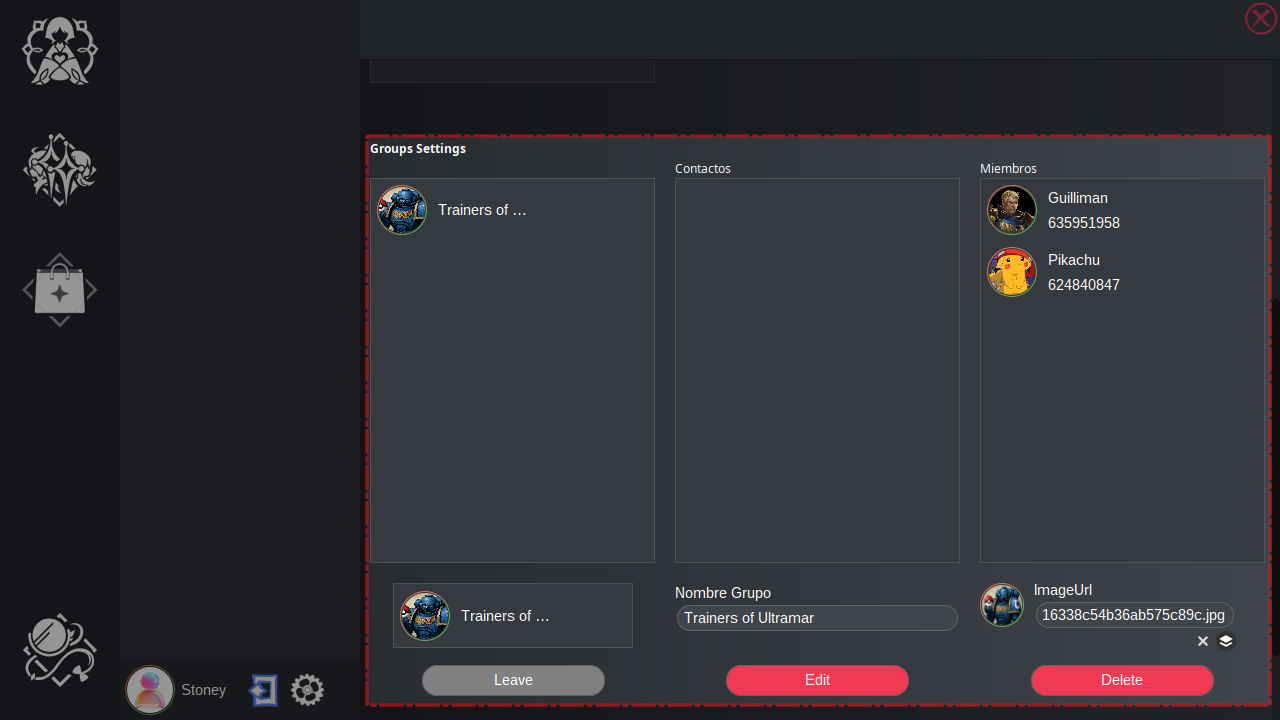
\includegraphics[width=0.58\textwidth]{images/manualDeUsuario/EditarContactos&Grupos3.png}
    \caption*{Ajustes de grupos}
\end{figure}

\subsection*{8. Buscar mensajes}
Para buscar mensajes, el usuario debe pulsar el botón correspondiente para acceder a la pantalla de búsqueda.  
Puede buscar mensajes combinando Número de teléfono, Nombre de contacto y un fragmento de texto.

\begin{itemize}
    \item Número de teléfono
    \item Nombre de contacto
    \item Fragmento de texto
\end{itemize}

Los resultados se muestran tanto en una lista sin formato para una búsqueda rápida, como en una vista renderizada para una mejor visualización.

\begin{figure}[H]
    \centering
    \begin{minipage}[b]{0.48\textwidth}
        \centering
        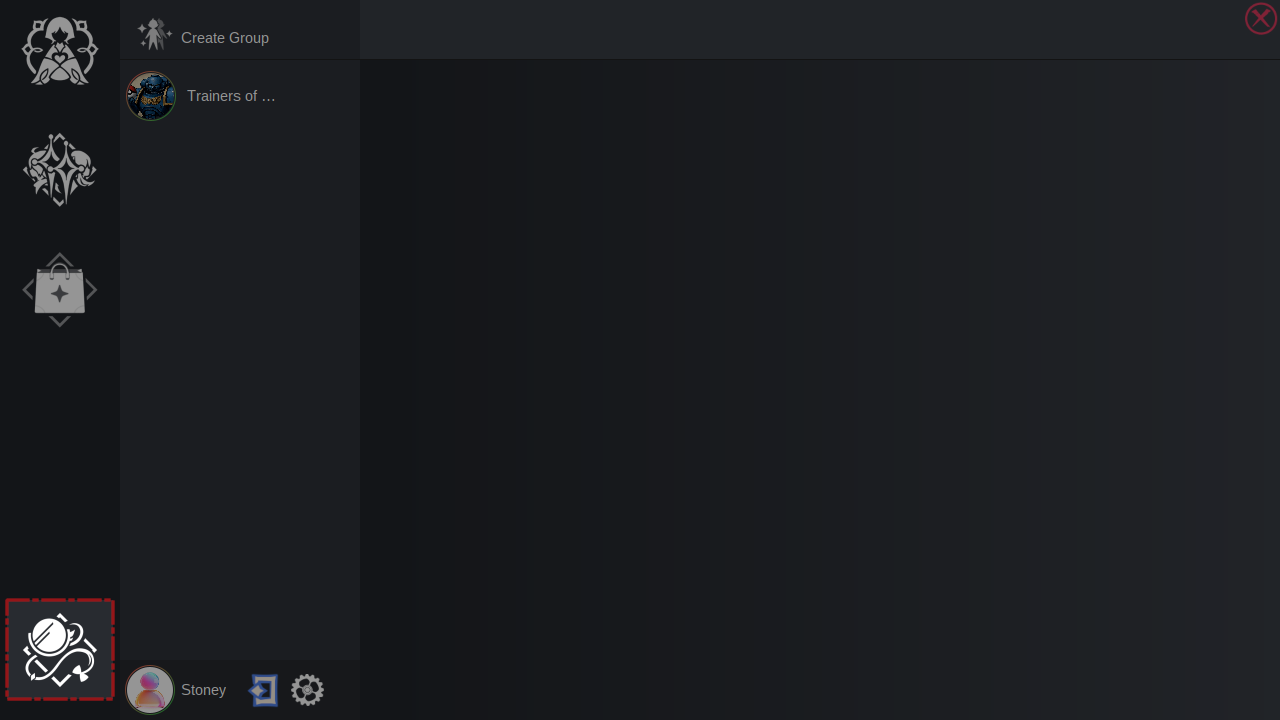
\includegraphics[width=\textwidth]{images/manualDeUsuario/BuscarMensajes1.png}
        \caption*{Botón de búsqueda}
    \end{minipage}
    \hfill
    \begin{minipage}[b]{0.48\textwidth}
        \centering
        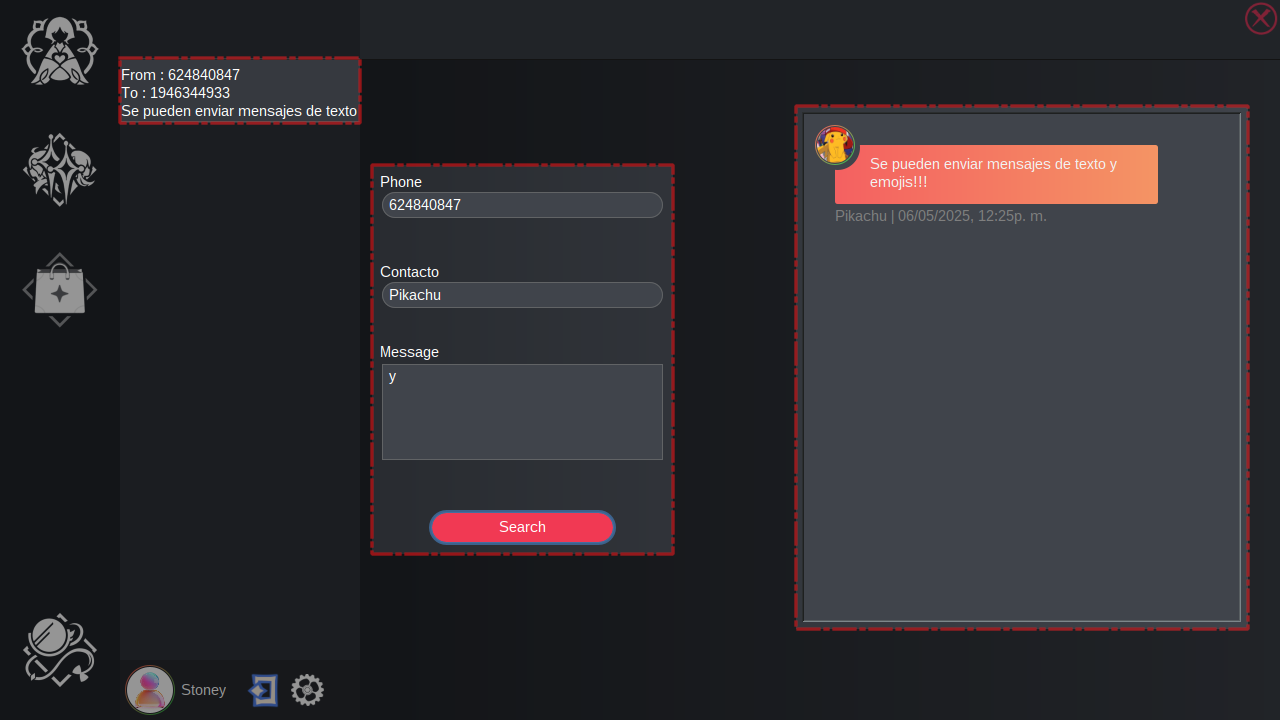
\includegraphics[width=\textwidth]{images/manualDeUsuario/BuscarMensajes2.png}
        \caption*{Pantalla de búsqueda}
    \end{minipage}
\end{figure}

\subsection*{9. Cerrar sesión}
Para cerrar sesión, se debe pulsar el botón de azul en la parte inferior de la pantalla principal.\\
Esto cerrará la sesión del usuario y lo llevará de nuevo a la pantalla de inicio de sesión.

\begin{figure}[H]
    \centering
    \begin{minipage}[b]{0.5\textwidth}
        \centering
        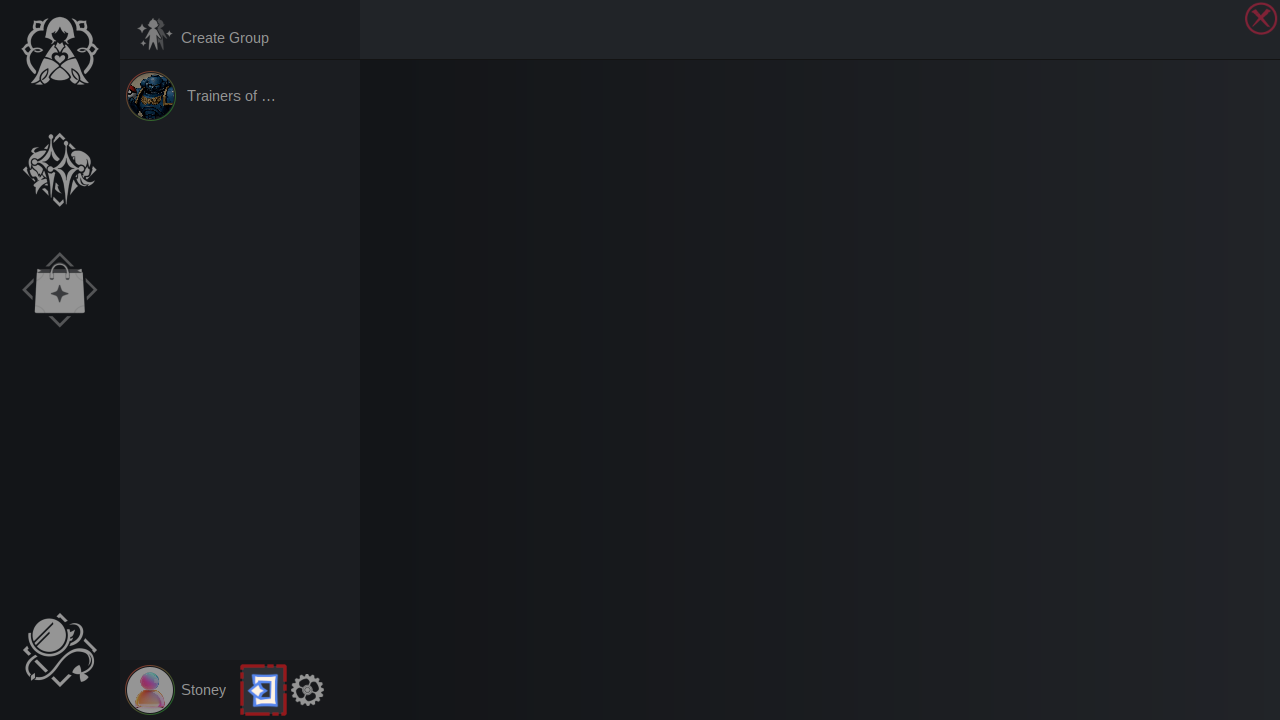
\includegraphics[width=\textwidth]{images/manualDeUsuario/Logout1.png}
        \caption*{Botón de cerrar sesión}
    \end{minipage}
    \hfill
    \begin{minipage}[b]{0.48\textwidth}
        \centering
        \includegraphics[width=\textwidth]{images/manualDeUsuario/InicioAplicación.png}
        \caption*{Pantalla de inicio de sesión}
    \end{minipage}
\end{figure}

\newpage

\subsection*{10. Comprar Premium}
Para acceder a la opción de compra de la versión Premium, el usuario debe pulsar el botón de la tienda en la pantalla principal.

\begin{figure}[H]
    \centering
    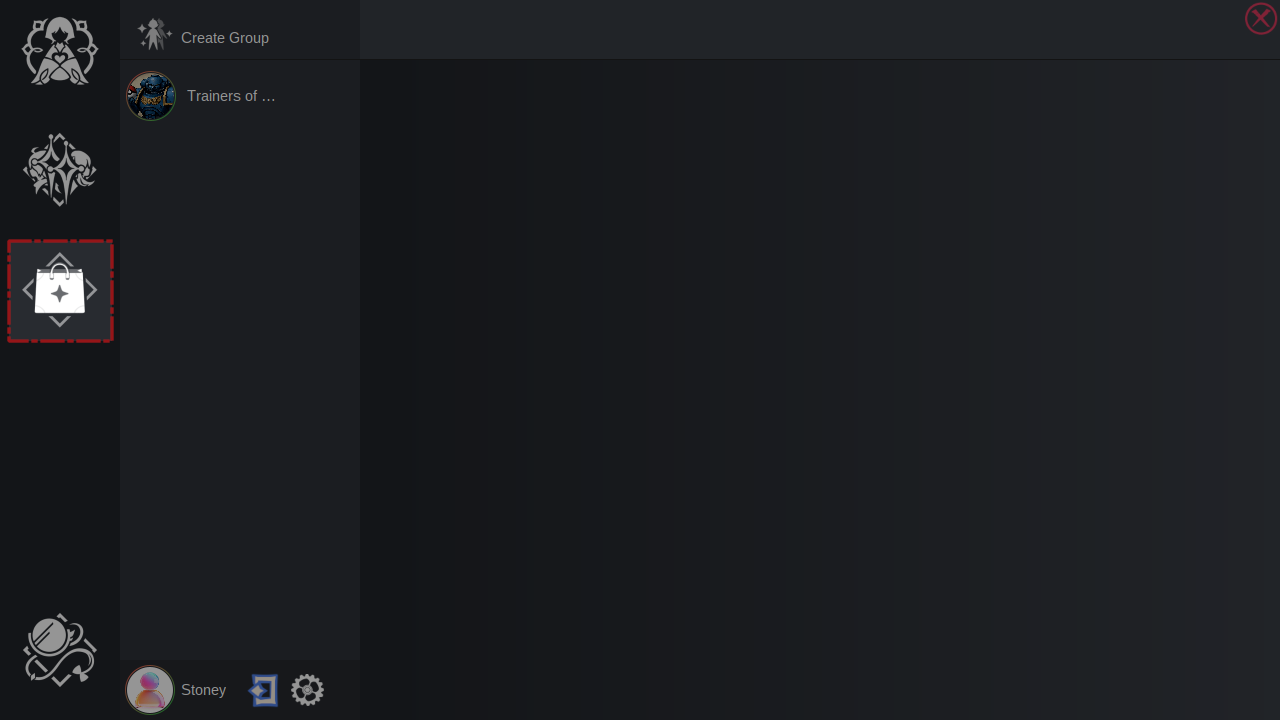
\includegraphics[width=0.48\textwidth]{images/manualDeUsuario/HacerPremium1.png}
    \caption*{Botón de tienda}
\end{figure}

Una vez en la tienda debe elegir una de las opciones disponibles y pulsar el botón \texttt{Buy Premium}.

\begin{figure}[H]
    \centering
    \begin{minipage}[b]{0.48\textwidth}
        \centering
        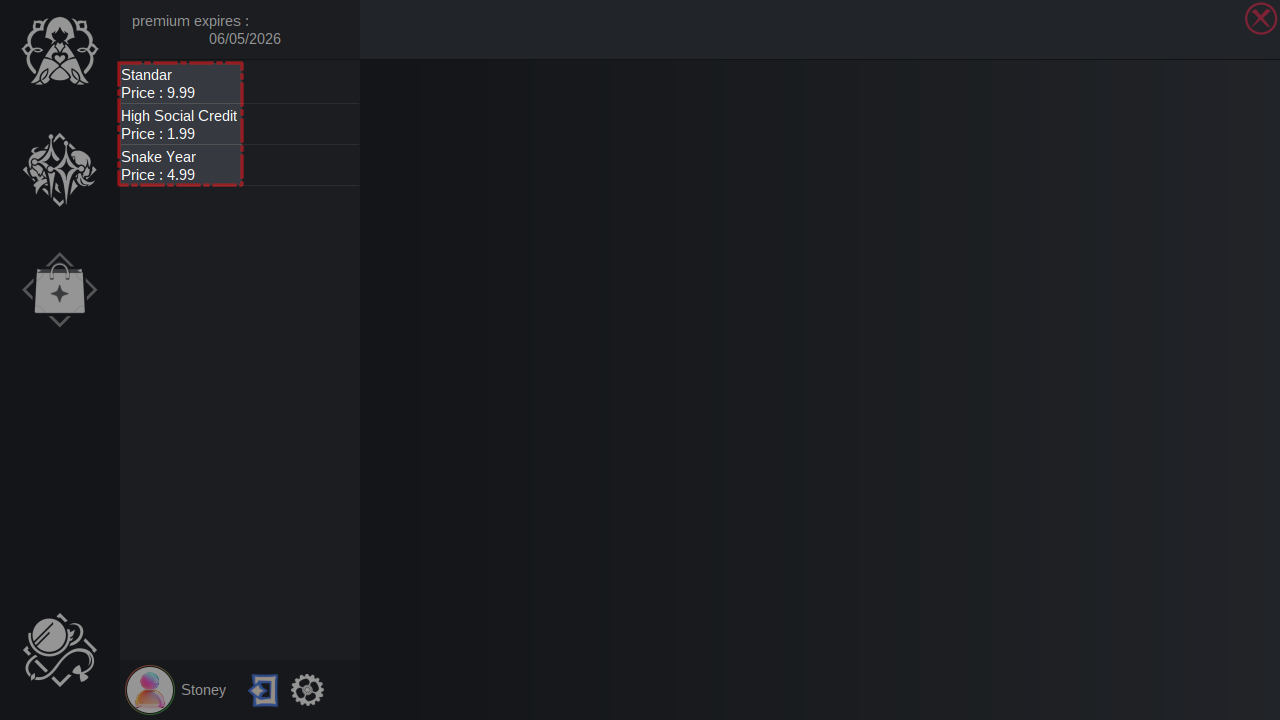
\includegraphics[width=\textwidth]{images/manualDeUsuario/HacerPremium2.png}
        \caption*{Listado de ofertas}
    \end{minipage}
    \hfill
    \begin{minipage}[b]{0.48\textwidth}
        \centering
        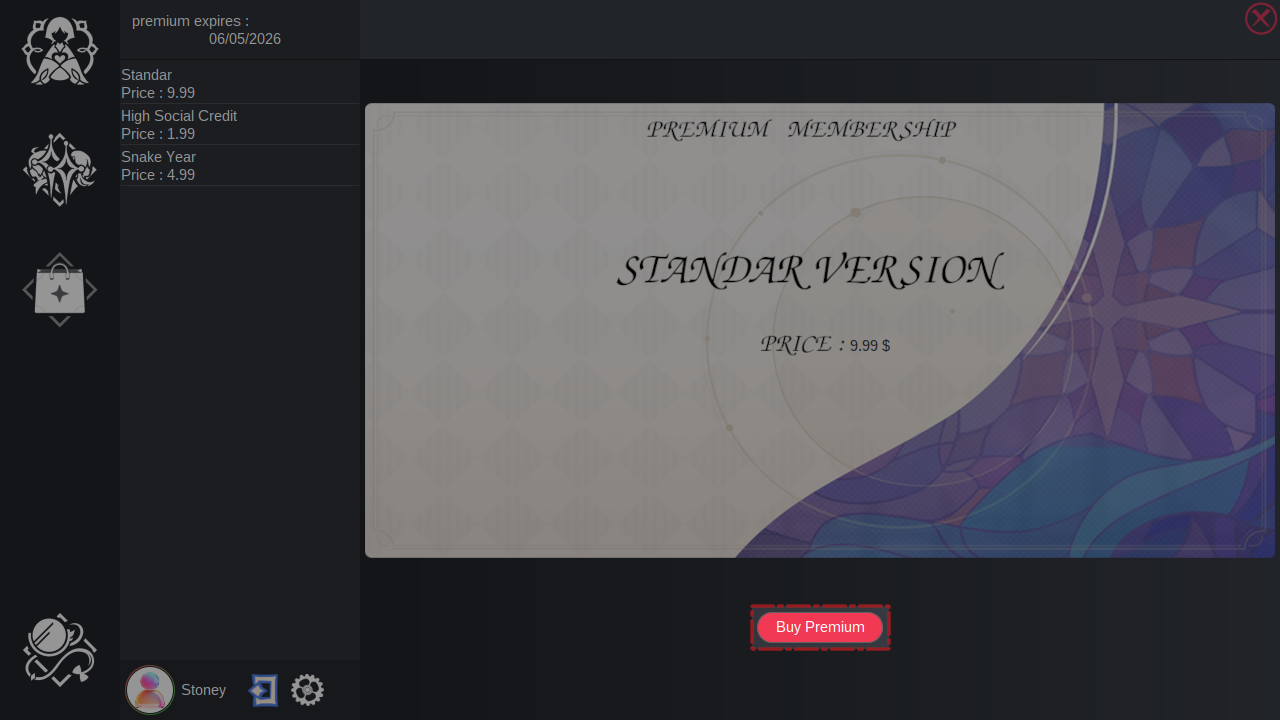
\includegraphics[width=\textwidth]{images/manualDeUsuario/HacerPremium3.png}
        \caption*{Pantalla de compra}
    \end{minipage}
\end{figure}

\subsection*{11. Exportar mensajes a PDF}
Para exportar los mensajes a PDF, el usuario debe pulsar el botón \texttt{Export to PDF} en la pantalla de ajustes.\\
Solo los usuarios premium pueden utilizar esta función.\\
No está permitido exportar mensajes de grupos, ya que en ellos participan varios usuarios.\\
El archivo se genera en el directorio base del usuario.

\begin{figure}[H]
    \centering
    \begin{minipage}[b]{0.48\textwidth}
        \centering
        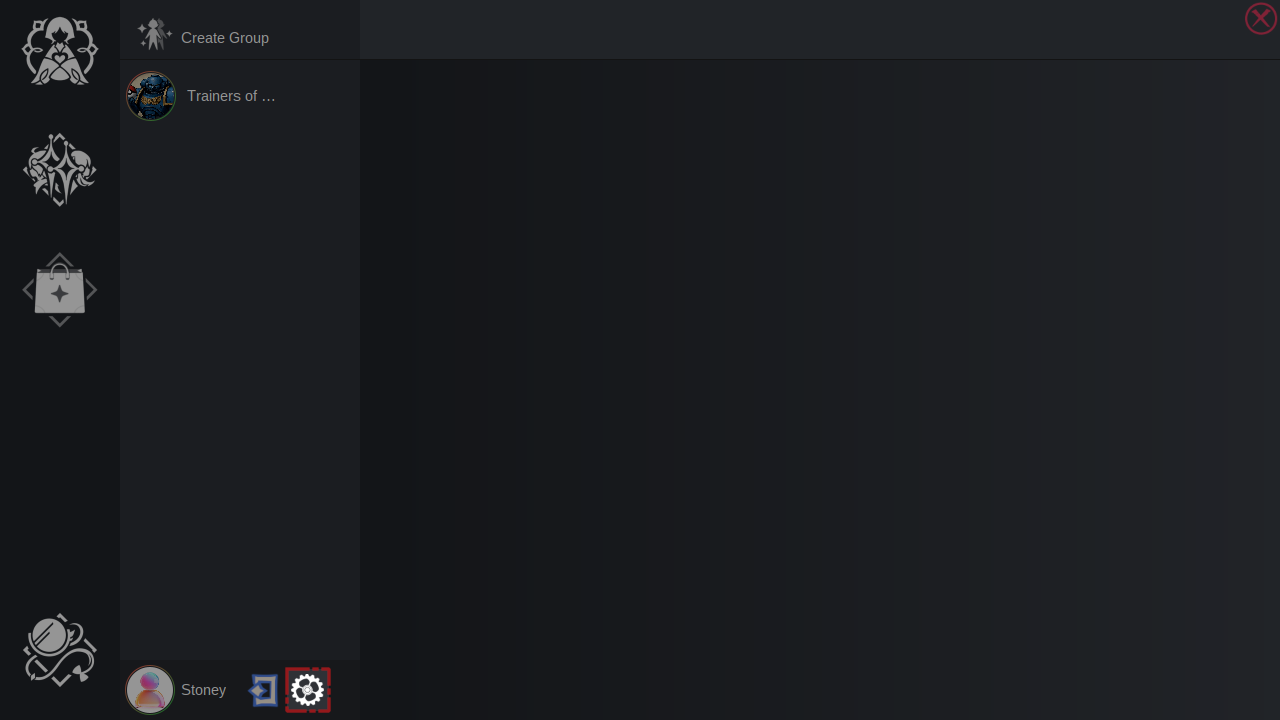
\includegraphics[width=\textwidth]{images/manualDeUsuario/EditarContactos&Grupos1.png}
        \caption*{Botón de ajustes}
    \end{minipage}
    \hfill
    \begin{minipage}[b]{0.48\textwidth}
        \centering
        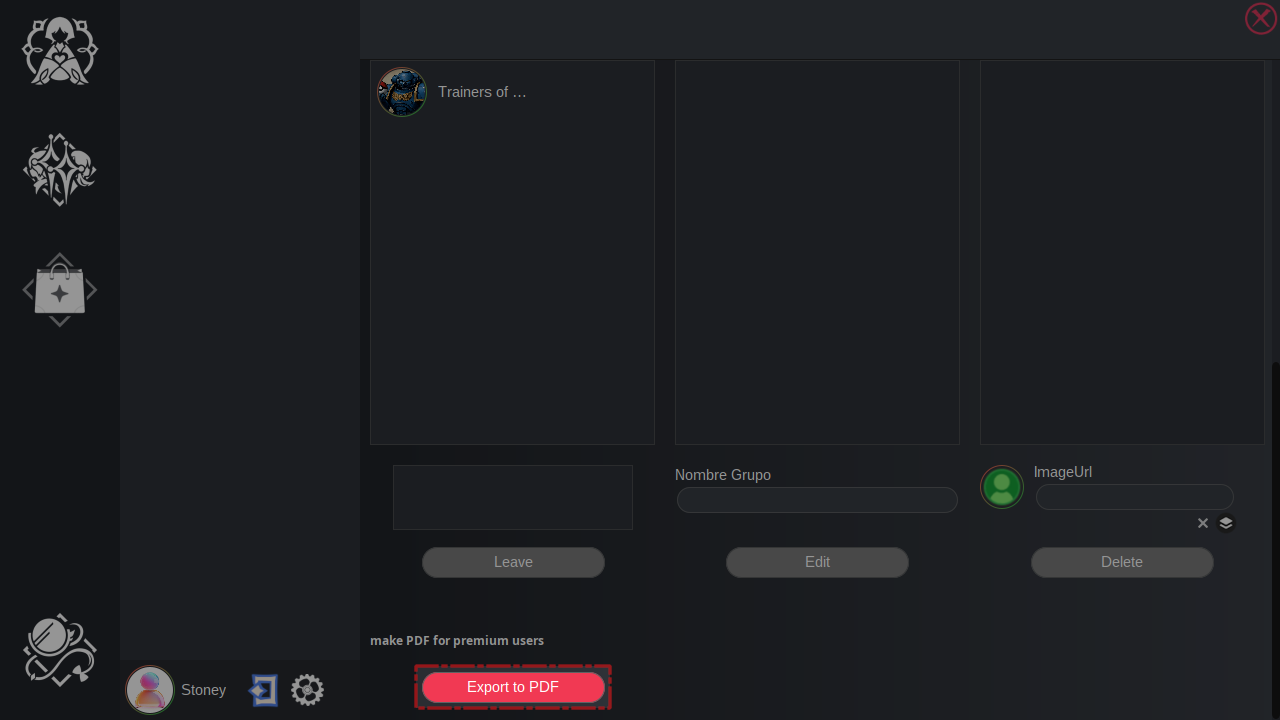
\includegraphics[width=\textwidth]{images/manualDeUsuario/ExportarAPDF1.png}
        \caption*{Botón de exportar a PDF}
    \end{minipage}
\end{figure}